\documentclass{beamer}
\usetheme{focus}
\usepackage[utf8]{inputenc}
\usepackage{polski}
\usepackage{amsfonts}
\usepackage{amsmath}
\usepackage{natbib}
\usepackage{graphicx}
\usepackage{array,booktabs,tabularx}
\usepackage{epstopdf}
\usepackage{colortbl, xcolor}
\usepackage{url}

\definecolor{main}{RGB}{92, 138, 168}
\definecolor{background}{RGB}{240, 247, 255}

\title{AmyloGram 2.0: MBO in the prediction of amyloid proteins}
\date{}
\author{Dominik Rafacz}
\institute{Warsaw University of Technology}

\usepackage{Sweave}
\begin{document}
\Sconcordance{concordance:presentation.tex:presentation.Rnw:%
1 18 1 1 0 54 1}



\maketitle
\begin{frame}{Amyloidogenic proteins}
  \begin{figure} 
    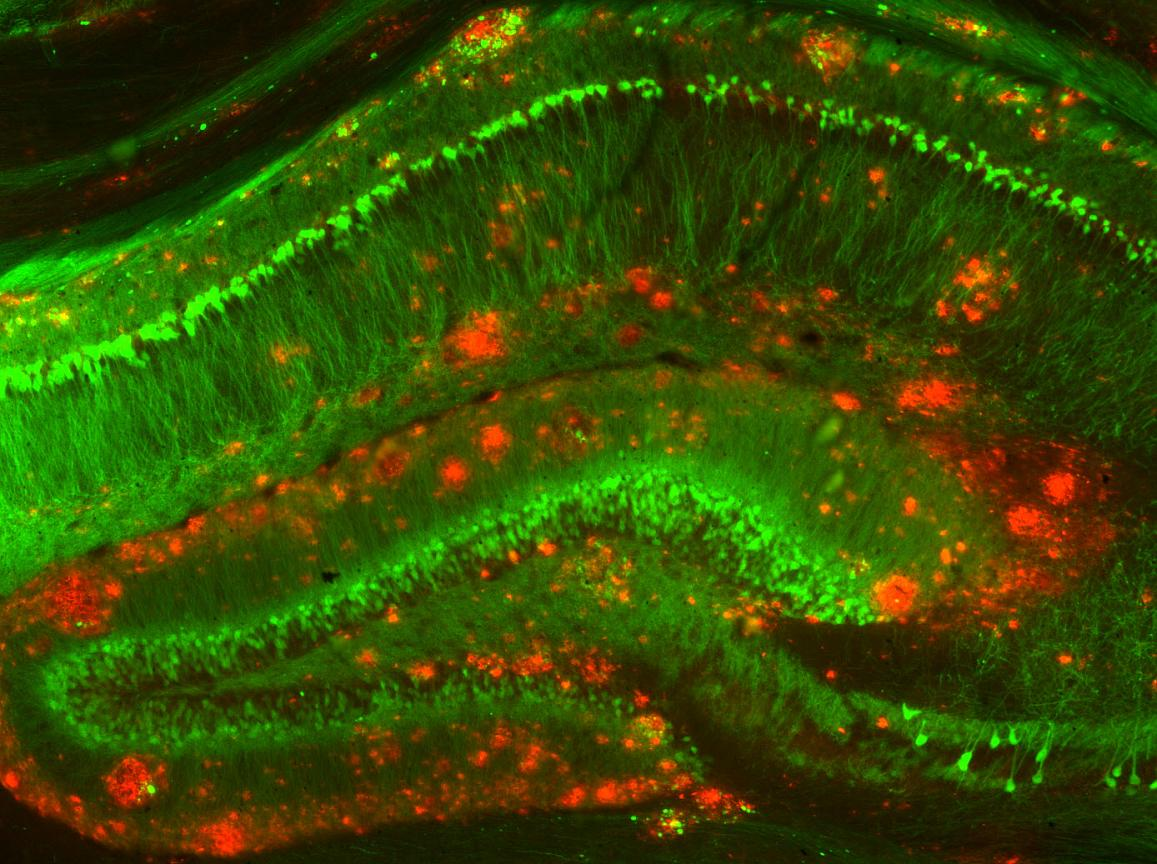
\includegraphics[width=0.75\textwidth]{figures/amyloid_aggregates.jpg}
  \end{figure}
  
  \footnotesize
  Amyloid aggregates (red) around neurons (green). Strittmatter Laboratory, Yale University.
\end{frame}


\begin{frame}{AmyloGram - n-grams analysis}
  \begin{figure} 
    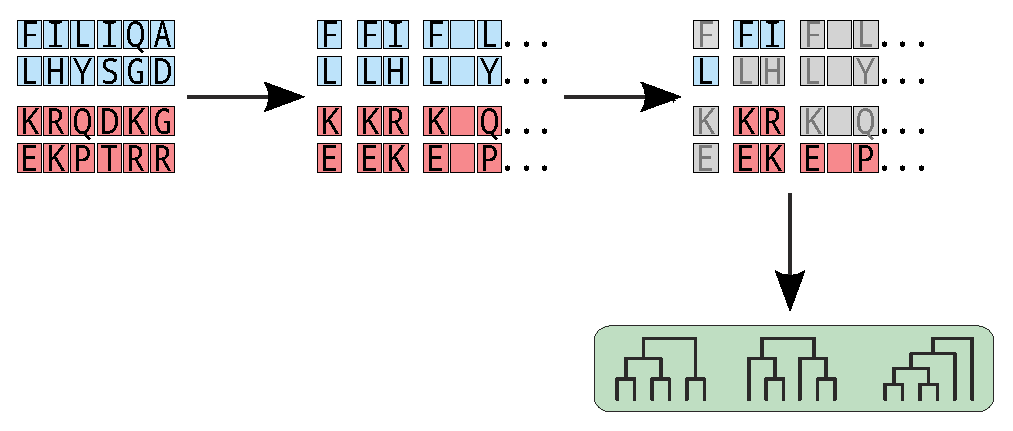
\includegraphics[width=0.95\textwidth]{figures/ngram1.eps}
  \end{figure}
  
  Example 1-grams: A, L, G \\
  Example 2-grams: AL, MM, MY \\
  Example 2-grams (with a gap): A-L, M-M, M-Y
  
  \begin{tiny}
    Burdukiewicz, M., Sobczyk, P., Rödiger, S., Duda-Madej, A., Mackiewicz, P., and Kotulska, M. (2017). Amyloidogenic motifs revealed by n-gram analysis. Scientific Reports 7, 12961 \\
  \end{tiny}
\end{frame} 


\begin{frame}{AmyloGram - alphabet reduction}
  \begin{figure} 
    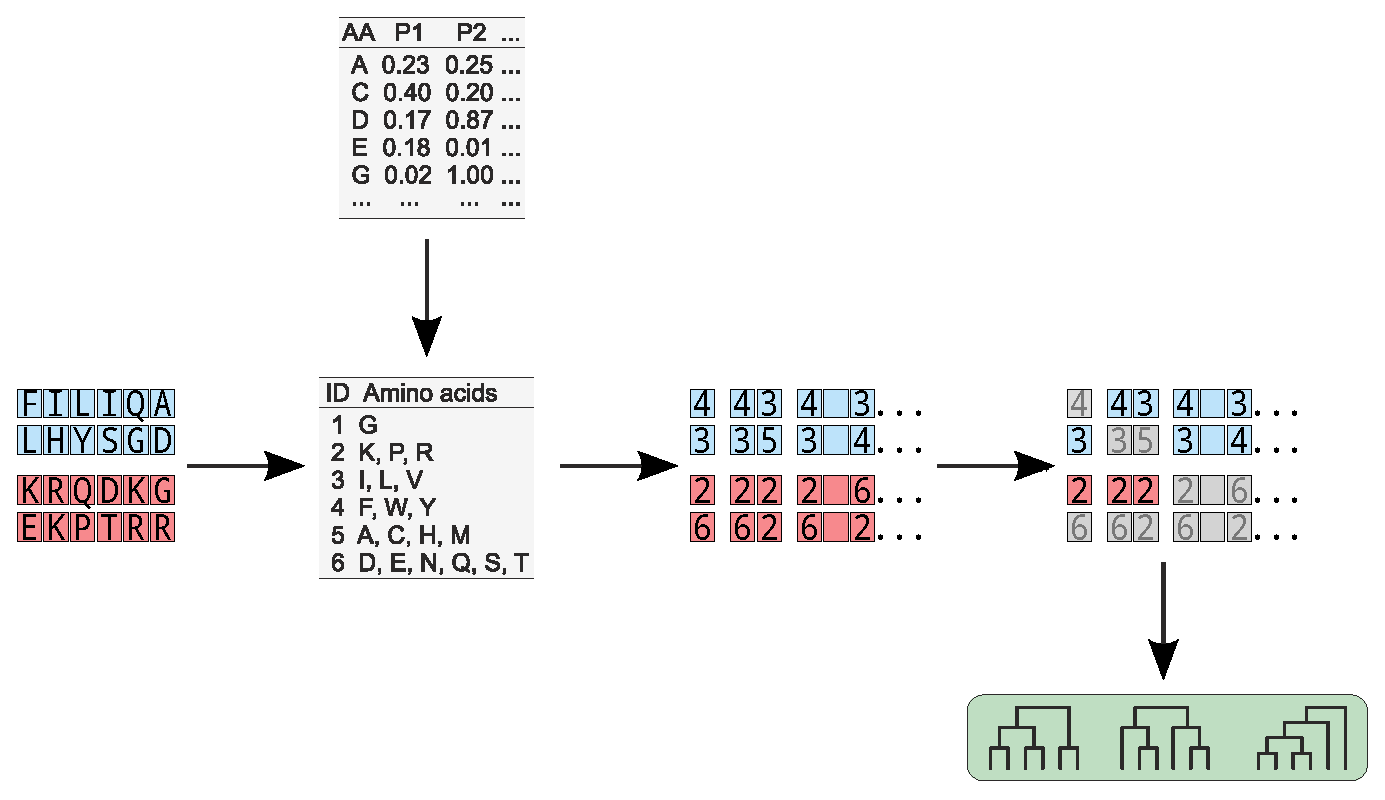
\includegraphics[width=0.95\textwidth]{figures/ngram3.eps}
  \end{figure}

  \tiny{Burdukiewicz, M., Sobczyk, P., Rödiger, S., Duda-Madej, A., Mackiewicz, P., and Kotulska, M. (2017). Amyloidogenic motifs revealed by n-gram analysis. Scientific Reports 7, 12961}
\end{frame}


\begin{frame}{MBO}

\end{frame} 

\begin{frame}{Results}

\end{frame} 

\begin{frame}{Acknowledgements}

\end{frame} 

\begin{frame}{References}

\end{frame} 
\end{document}
